\section{Experiments}\label{se-exp}

\begin{figure*}[!tb]
\centering
    \phantom{\,}%
    \hfill%
    $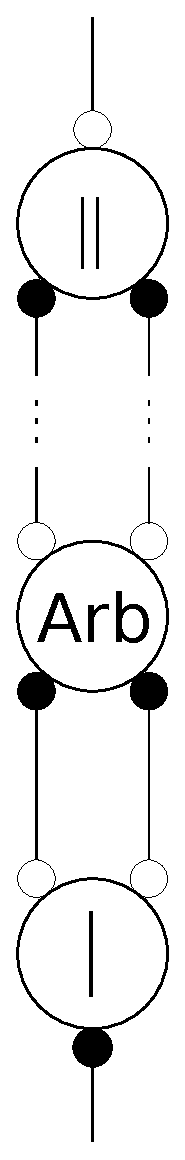
\includegraphics[scale=0.3]{fig/par_arb_mix}
    \atop
    \mbox{\rule[1.3em]{0em}{0em}\ParArbCall}$%
    \hfill%
    $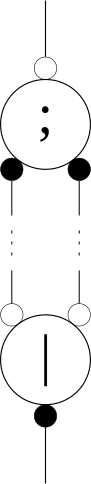
\includegraphics[scale=0.3]{fig/seq_mix}
    \atop
    \mbox{\rule[1.3em]{0em}{0em}\SeqCall}$%
    \hfill%
    $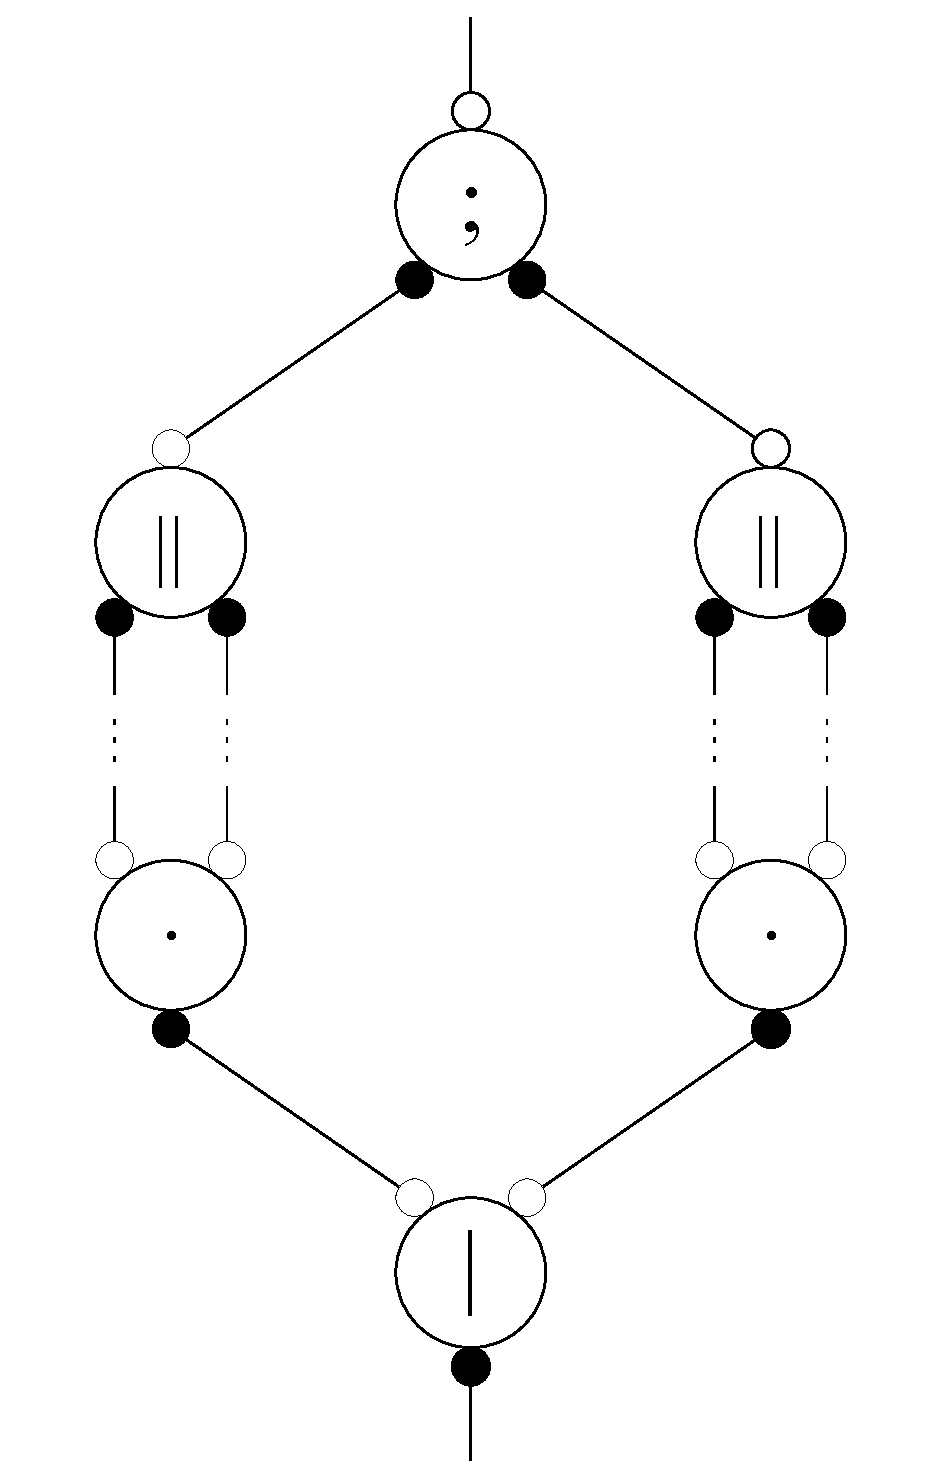
\includegraphics[scale=0.3]{fig/seq_par_sync_mix}
    \atop
    \mbox{\rule[1.3em]{0em}{0em}\SeqCallParSync}$%
    \hfill%
    \phantom{\,}%
    \\
    \caption{\label{fig:Scalable-Balsa-controllers}
        Scalable Balsa controllers used in experiments.
    }
\end{figure*}

\begin{figure*}[p]
\centering

  \subfloat[All contractions]{
    \shortstack[l]{
    $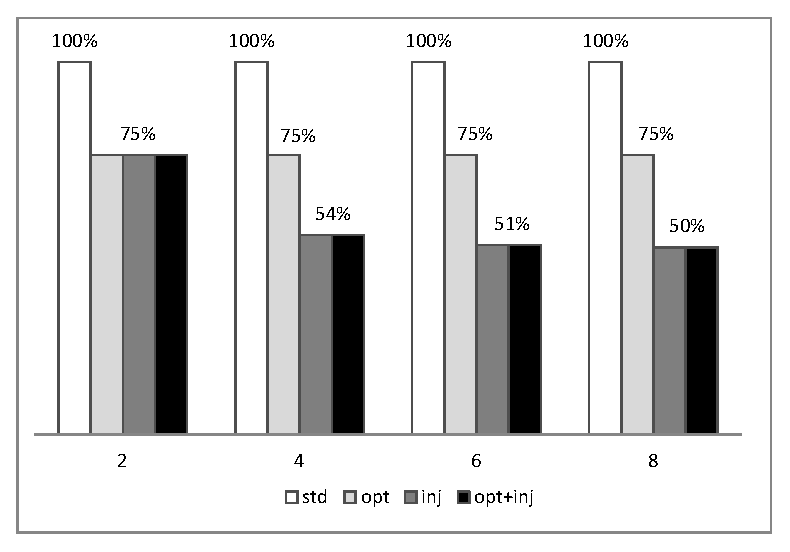
\includegraphics[width=0.48\textwidth]{fig/ParArbMix_all}
    \atop
    \mbox{\rule[1.3em]{0em}{0em}\ParArbCall}$%
    \\[1em]
    $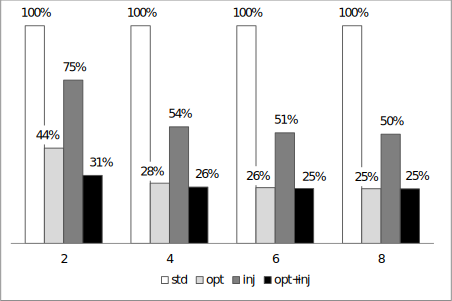
\includegraphics[width=0.48\textwidth]{fig/SeqMix_all}
    \atop
    \mbox{\rule[1.3em]{0em}{0em}\SeqCall}$%
    \\[1em]
    $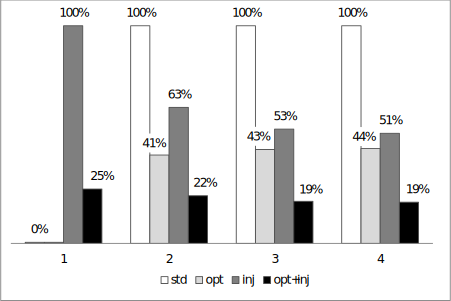
\includegraphics[width=0.48\textwidth]{fig/SeqMixParSync_all}
    \atop
    \mbox{\rule[1.3em]{0em}{0em}\SeqCallParSync}$%
    }
    }
    \hfill%
  \subfloat[Safeness-preserving contractions]{
    \shortstack[l]{
    $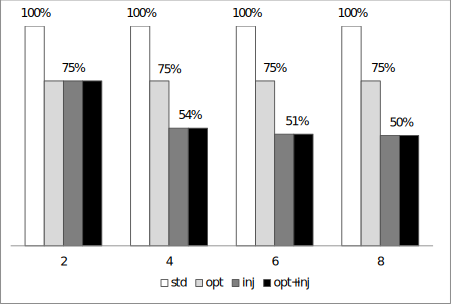
\includegraphics[width=0.48\textwidth]{fig/ParArbMix_safe}
    \atop
    \mbox{\rule[1.3em]{0em}{0em}\ParArbCall}$%
    \\[1em]
    $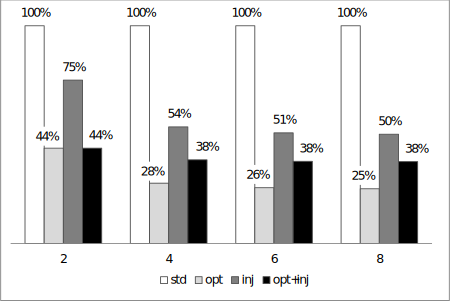
\includegraphics[width=0.48\textwidth]{fig/SeqMix_safe}
    \atop
    \mbox{\rule[1.3em]{0em}{0em}\SeqCall}$%
    \\[1em]
    $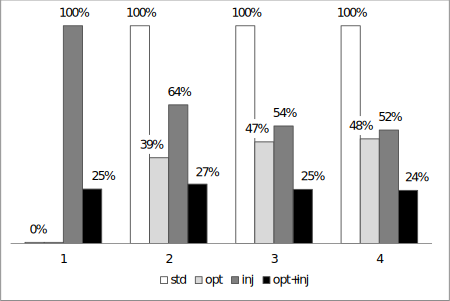
\includegraphics[width=0.48\textwidth]{fig/SeqMixParSync_safe}
    \atop
    \mbox{\rule[1.3em]{0em}{0em}\SeqCallParSync}$%
    }}
    \caption{\label{fi-exp}
        Experimental results.
    }
\end{figure*}

The proposed parallel composition algorithm has been evaluated
on three series of scalable benchmarks (available
from~\cite{pcomp}), see
Fig.~\ref{fig:Scalable-Balsa-controllers}. They are built of a
subset of standard \balsa components~\cite{EB-02}:
Paralleliser~$(\parallel)$, Sequencer~$(;)$, Call~$(|)$,
Synchroniser~$(\cdot)$ and Arbiter~(Arb). These controllers are
considered to be of size~1; a controller of size~$k>1$ is
constructed by replacing the dotted lines with the controllers
of size~$k-1$. Each basic component is described by an
individual STG; then these STGs are composed using four
different techniques:
\begin{description}
  \item[std] the standard parallel composition;
  \item[opt] the optimised parallel composition presented
      here;
  \item[inj] the standard parallel composition of the
      components with enforced injective labelling;
  \item[opt+inj] the optimised parallel composition of the
      components with enforced injective labelling.
\end{description}
Note that all the used \balsa components except Call initially
had injective labelling, so only the STG for Call was changed
in the inj and opt+inj series. Both the standard and optimised
parallel composition algorithms have been implemented in \pcomp
tool~\cite{pcomp}. The tool automatically deletes duplicate
places in all compositions, so all the experimental results are
subject to this simplification. The runtimes of \pcomp were
negligible and so not reported.

For each composed STG, the internal signals of the composition
were hidden (\ie turned into dummies), and the \desij
tool~\cite{DesiJ} was used to structurally eliminate as many
dummies as possible, using either secure or safeness-preserving
secure contractions.

The results of our experiments are summarised by the charts in
Fig.~\ref{fi-exp}. There are six charts altogether, for each of
the three benchmark series and each of the contraction modes
(secure or safeness-preserving secure). Each chart reports, for
each benchmark size within the corresponding series, the
numbers of non-con\-trac\-tible dummy transitions (normalised
\wrt the worst result) remaining in the STG for each of the
four composition methods described above.

The experiments demonstrate that the optimised parallel
composition is never worse than the standard one in terms of
the STG structure that is used for removing dummies (the opt
bars are never longer than the std bars, and the opt+inj bars
are never longer than the inj bars), and is significantly
better in some cases (\eg for the \SeqCallParSync(4) benchmark
there is a factor of five improvement). Moreover, using the
optimised technique in conjunction with injective labelling is
usually advantageous (the fourth bar is the shortest in almost
all cases).
